  %-------------------------------------------------------------------------------
%-------------------------------------------------------------------------------
%-------------------------------------------------------------------------------
\chapter{Équations différentielles}
%-------------------------------------------------------------------------------
%-------------------------------------------------------------------------------
\thispagestyle{empty}
\begin{itemize}
    \item Dans le TP la variable des fonctions sera représentée par $t$. En particulier les équations différentielles seront sous la forme $y' = \varphi(y, t)$.
    \item Il arrivera que la variable $t$ n'apparaisse pas directement dans l'équation : on devra néanmoins la faire intervenir dans la fonction python \type{def phi(y, t)}.
    \item Les fonctions mathématiques seront importées depuis le module \type{math}
\begin{lstlisting}
import math as m
\end{lstlisting}
    \item Lors de cette étude nous allons régulièrement tracer le graphe des solutions.

On aura calculé la liste des abscisses : \type{T} et la liste des valeurs approchées d'une fonction : \type{Y}.

Pour tracer le graphe on utilise le module \type{matplotlib}.
\begin{lstlisting}
import matplotlib.pyplot as plt
plt.plot(X, Y)
plt.show()
\end{lstlisting}
\item Lorsque l'on trace plusieurs graphes dans un même cadre, on pourra donner une étiquette à chacun :
\begin{lstlisting}
plt.plot(T, Y, label = "Ma jolie fonction")
\end{lstlisting}
et faire afficher ces étiquette par \type{plt.legend()}.
\item Des fonctions supplémentaires sont données dans le document du concours centrale.
\end{itemize}
%--------------------------------------------------------------------------
%--------------------------------------------------------------------------
%--------------------------------------------------------------------------
\section{Outils de base}
%-------------------------------------------------------------------------------
%-------------------------------------------------------------------------------
%-------------------------------------------------------------------------------
\begin{Exercise}\it
Écrire une fonction \type{listeT(a, b, n)} qui calcule une liste de longueur $n$ dont les valeurs sont équiréparties entre $a$ et $b$.
\end{Exercise}
%-------------------------------------------------------------------------------
\begin{Answer}
\begin{lstlisting}
def listeT(a, b, n):
    pas = (b-a)/(n-1)
    T = [0]*n
    for k in range(n):
        T[k] = a + k*pas 
    return T
\end{lstlisting}
\end{Answer}
%-------------------------------------------------------------------------------
\smallskip
\type{listeT(1, 3, 5)} doit renvoyer \type{[1.0, 1.5, 2.0, 2.5, 3.0]}.

On remarquera que le pas est $\frac{b-a}{n-1}$.
%-------------------------------------------------------------------------------
%-------------------------------------------------------------------------------
\begin{Exercise}\it
Écrire une fonction \type{appliquer(f, T)} où $f$ est une fonction et $T$ est une liste et qui renvoie une liste $Y$ de même longueur que $T$ telle que \type{Y[i] = f(T[i])}.
\end{Exercise}
%-------------------------------------------------------------------------------
\begin{Answer}
\begin{lstlisting}
def appliquer(f, T):
    n = len(T)
    Y = [0]*n
    for i in range(n):
        Y[i] = f(T[i])
    return Y
\end{lstlisting}
\end{Answer}
%-------------------------------------------------------------------------------
\smallskip
Pour la fonction $f$ : $x \mapsto 3x+1$,  \type{appliquer(f, [0, 1, 2])} doit renvoyer \type{[1, 4, 7]}.
%--------------------------------------------------------------------------
%--------------------------------------------------------------------------
%--------------------------------------------------------------------------
\section{Méthode d'Euler}
%--------------------------------------------------------------------------
%--------------------------------------------------------------------------
%--------------------------------------------------------------------------
On rappelle la fonction de calcul de solution par la méthode d'Euler.
%--------------------------------------------------------------------------
\begin{lstlisting}
def euler(phi, y0, T):
    """Entrée : phi : fonction de ExR vers E 
                y0 élément de E, la condition initiale y0
                T : une liste d'abscisses
       Sortie : une solution approchée de y' = f(t,y)
                avec les conditions initiales (T[0],y0)
                sous la forme d'une liste des valeurs
                aux points de T"""
    n = len(T)
    Y = [0]*n
    Y[0] = y0 # ordonnée initiale
    for i in range(n-1): # il reste n-1 valeurs à calculer
        pas = T[i+1] - T[i]
        pente = phi(Y[i], T[i])  
        Y[i+1] = Y[i] + pas*pente
    return Y
\end{lstlisting}
%--------------------------------------------------------------------------
%--------------------------------------------------------------------------
\subsection{Un exemple simple}
%--------------------------------------------------------------------------
%--------------------------------------------------------------------------
On s'intéresse à l'équation $y' = y$, sur $[0; 1]$ avec $y(0) = 1$. La solution est $x\mapsto \exp(x)$.
%--------------------------------------------------------------------------
%--------------------------------------------------------------------------
\begin{Exercise}\it
Approcher les solutions de cette équation en utilisant la méthode d'Euler avec 5, 20 et 100 points.

On tracera aussi le graphe associé à \type{math.exp(t)} pour une liste de temps avec 100 points.
\end{Exercise}
%--------------------------------------------------------------------------
\begin{Answer}
\begin{lstlisting}
import math as m

def phi1(y, t) :
    return y

y0 = 1

T = listeT(0, 1, 5)
Y = euler(phi1, y0, T)
plt.plot(T, Y, label = "Euler avec 5 points")

T = listeT(0, 1, 20)
Y = euler(phi1, y0, T)
plt.plot(T, Y, label = "Euler avec 20 points")


T = listeT(0, 1, 100)
Y = euler(phi1, y0, T)
plt.plot(T, Y, label = "Euler avec 100 points")


T = listeT(0, 1, 100)
Y = appliquer(m.exp, T)
plt.plot(T, Y, label = "Solution exacte")

plt.legend()
plt.show()
\end{lstlisting}
\newpage
\end{Answer}
%--------------------------------------------------------------------------
%--------------------------------------------------------------------------
\begin{Exercise}\it
Dans l'exercice précédent, l'écriture naturelle est de répéter 3 fois les calculs ($T$, la solution, le graphe). Si c'est le cas, ré-écrire la solution en factorisant sous la forme :
\begin{lstlisting}
for n in [5, 20, 100]:
     T = 
     Y = 
     plt.plot
\end{lstlisting}

\end{Exercise}
%--------------------------------------------------------------------------
\begin{Answer}
\begin{lstlisting}
import math as m

def phi1(y, t) :
    return y

y0 = 1

for n in [5, 20, 100]:
    T = listeT(0, 1, n)
    Y = euler(phi1, y0, T)
    plt.plot(T, Y, label = "Euler avec {} points".format(n))

T = listeT(0, 1, 100)
Y = appliquer(m.exp, T)
plt.plot(T, Y, label = "Solution exacte")

plt.legend()
plt.show()
\end{lstlisting}
\end{Answer}
%--------------------------------------------------------------------------
%--------------------------------------------------------------------------

\medskip

Comme on connaît la solution exacte, on peut mesurer l'erreur commise par la méthode.

On admet que l'erreur est maximale pour $t=1$.
%--------------------------------------------------------------------------
%--------------------------------------------------------------------------
\begin{Exercise}[title = {Qualité de l'approximation}]\it
Écrire les instructions qui permettent d'afficher à l'écran la valeur absolue entre \type{m.exp(1)} et le dernier terme de la liste retournée par la fonction \type{euler} pour des listes de $10^p$ points avec $p\in \{1, 2, 3, 4, 5,6, 7\}$.
\end{Exercise}
%--------------------------------------------------------------------------
\begin{Answer}
\begin{lstlisting}
import math as m

def phi1(y, t) :
    return y

y0 = 1

for n in [5, 20, 100]:
    T = listeT(0, 1, n)
    Y = euler(phi1, y0, T)
    plt.plot(T, Y, label = "Euler avec {} points".format(n))

T = listeT(0, 1, 100)
Y = appliquer(m.exp, T)
plt.plot(T, Y, label = "Solution exacte")

plt.legend()
plt.show()
\end{lstlisting}
\end{Answer}
%--------------------------------------------------------------------------
%--------------------------------------------------------------------------
\begin{Exercise}[title = {Revenir en arrière}]\it
Tracer la solution de l'équation sur $[-1;0]$
\end{Exercise}
%--------------------------------------------------------------------------
\begin{Answer}
\begin{lstlisting}
y0 = 1

T = listeT(0, -1, 1000)
Y = euler(phi1, y0, T)
plt.plot(T, Y)

plt.show()
\end{lstlisting}
\newpage
\end{Answer}
%--------------------------------------------------------------------------
%--------------------------------------------------------------------------
Le calcul est un peu long : on remarque que l'erreur est de l'odre de $\frac 1n$.
%--------------------------------------------------------------------------
%-------------------------------------------------------------------------------
\subsection{Étude d'un filtre actif passe bas}
%-------------------------------------------------------------------------------
%-------------------------------------------------------------------------------
\begin{minipage}[c]{0.45\linewidth}
On peut réaliser un filtre actif passe-bas avec un A.O. (Amplificateur opérationnel).

Le fonctionnement de l'amplificateur opérationnel implique que la tension de sortie, $u_s$, est solution de 
\[{R_1C} y'(t)+y(t) =  \frac{R_2+R_3}{R_2} u_e(t)\]

où $u_e$ est la tension d'entrée.
\end{minipage}
%-------------------------------------------------------------------------------
\hfill
%-------------------------------------------------------------------------------
\begin{minipage}[c]{0.55\linewidth}
%\shorthandoff{:!}
\begin{circuitikz}[scale=0.7]
\draw (5.2,1) node [op amp] (opamp) {};
\draw (-1,1) node[left] {$u_e$}to [R, l = $R_1$, o-*] (2,1);
\draw (2,1) -| (opamp.-);
\draw (2,1) to [C, l=$C$] (2,-4) node [ground] {};
\draw (opamp.+) -|  (3.5,-1) to [short, -*] (3.5,-1.5) to [R, l = $R_2$] (3.5,-4) node [ground] {};
\draw (opamp.out) to [short,-*]  (7,0.4) -- (8,0.4) node[ right] {$u_s$};
\draw (3.5,-1.5) to [R, l = $R_3$] (6.5,-1.5) -|  (7,0.5);
\end{circuitikz}
%\shorthandon{:!}
\end{minipage}
%-------------------------------------------------------------------------------

\medskip

Les valeurs numériques sont les suivantes :$R_2=R_3= 1000 \Omega$ et $C = 1 \mu $F.

Différentes valeurs de $R_1$ seront testées afin de mettre en évidence les différents comportements.

Le signal d'entrée $u_e(t)$ est un signal rectangulaire de fréquence 500 Hz.
%-------------------------------------------------------------------------------
\begin{center}
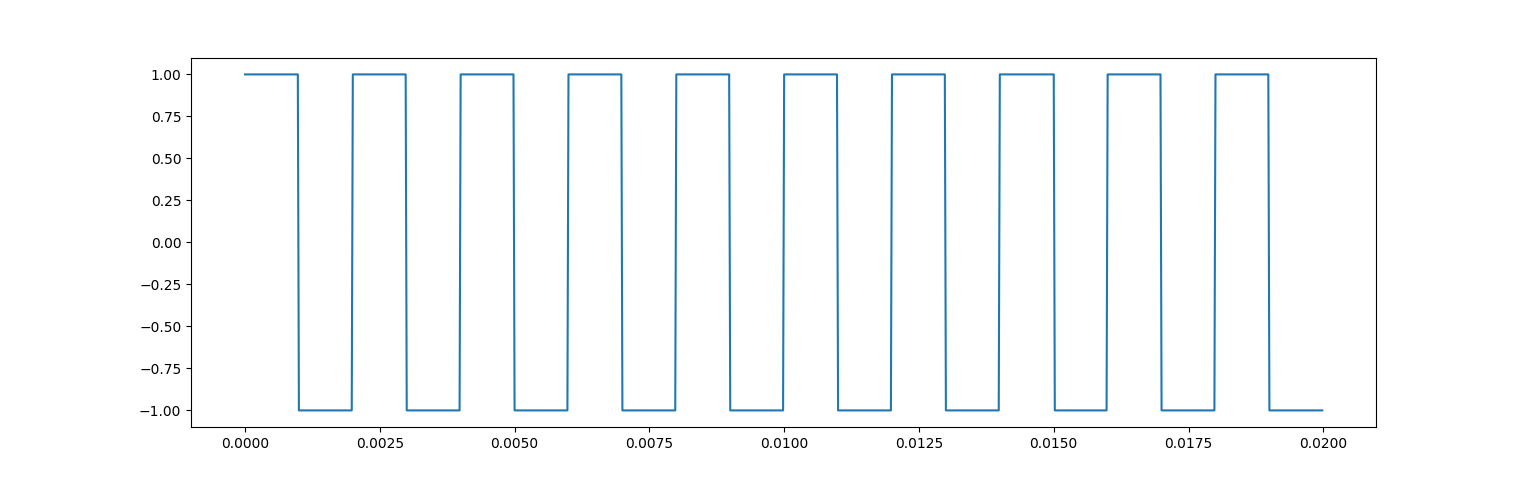
\includegraphics[width=13cm]{eu_rectangle.png}
\end{center}
%-------------------------------------------------------------------------------
%-------------------------------------------------------------------------------
\begin{Exercise}\it
Écrire une fonction \type{creneau(t,T)} qui calcule la valeur d'un signal rectangulaire de période $T$ : la valeur devra être 1 sur $[0;\frac T2[$ et $-1$ sur $[\frac T2;T[$.

\end{Exercise}
%-------------------------------------------------------------------------------
\begin{Answer}
\begin{lstlisting}
def creneau(t, T):
    x = t%T
    if x < T/2:
        return 1
    else:
        return -1
\end{lstlisting}
\end{Answer}
%-------------------------------------------------------------------------------
On pourra utiliser l'expression \type{t\%T} qui renvoie le réel $x$ appartenant à $[0;T[$ tel que $t-x$ est un multiple entier de $T$.
%-------------------------------------------------------------------------------
\begin{Exercise}\it
En utilisant la méthode d'Euler déterminer alors les solutions de l'équation : on prendra une liste de temps de 1000 points entre 0 et 0,01s avec une condition initiale nulle. 

On calculera les solutions pour $R_1=100\Omega$, $R_1=200\Omega$, $R_1=500\Omega$, $R_1=1000\Omega$ et $R_1=2000\Omega$. 

On pourra tracer les solutions en même temps que le signal d'entrée.
\end{Exercise}
%-------------------------------------------------------------------------------
\begin{Answer}
\begin{lstlisting}
def filtre(y, t):
    return ((R2 + R3)/R2*creneau(t, per) - y)/R1/C
\end{lstlisting}

\begin{lstlisting}
R2 = 1000
R3 = 1000
f = 500
per = 1/f
C = 1e-6
T = listeT(0, 0.01, 1000)
for R1 in [100, 200, 500, 1000, 2000]:
    Y = Euler(filtre, 0, T)
    plt.plot(T, Y, label = "$R_1$ = {}".format(R1))
    
def cr(t):
    return creneau(t, per)
Y = appliquer(cr, T)
plt.plot(T, Y, label = "Entrée")
plt.legend()
plt.show()
\end{lstlisting}
\begin{center}
	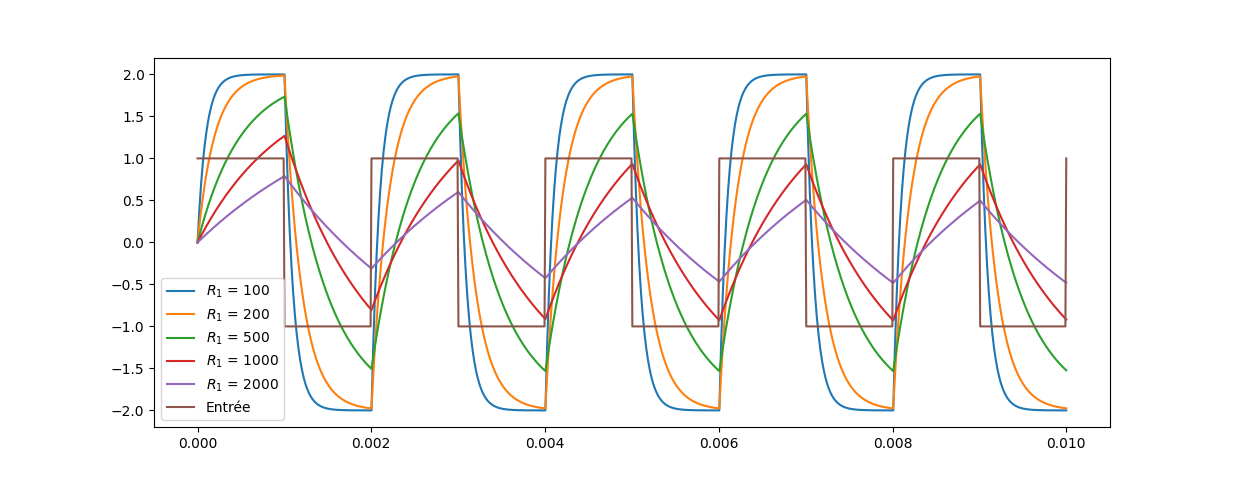
\includegraphics[width = 15cm]{eu_passeBas.png}
\end{center}
\newpage
\end{Answer}
%-------------------------------------------------------------------------------
%-------------------------------------------------------------------------------
\subsection{Limites}
%-------------------------------------------------------------------------------
%-------------------------------------------------------------------------------
On considère l'équation différentielle $\displaystyle y' = y -\frac{t+2}{(t+1)^2}$ avec la condition initiale $y(0)=1$.
%-------------------------------------------------------------------------------
%-------------------------------------------------------------------------------
\begin{Exercise}[label = Modification de solution]\it
Résoudre l'équation et tracer la solution sur $[0;3]$, $[0;10]$ et $[0;30]$ avec 10\,000 points.

Commenter sachant que la solution est $t \mapsto \frac 1 {t+1}$ et que la solution générale est $t \mapsto C.e^t + \frac 1 {t+1}$. 
\end{Exercise}
%-------------------------------------------------------------------------------
\begin{Answer}
\begin{lstlisting}
y0 = 1
t_max = 30

T = listeT(0, t_max, 10000)
Y = euler(phi2, y0, T)
plt.plot(T, Y)
plt.show()
\end{lstlisting}
\begin{center}
	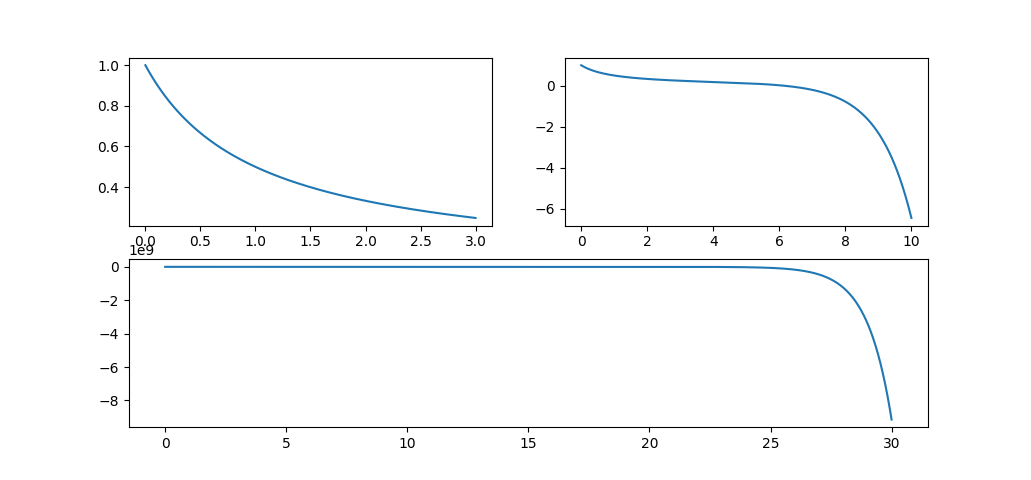
\includegraphics[width = 15cm]{eu_div.png}
\end{center}
Les erreurs d'arrondis des flottants font qu'on a en fait une solution $t \mapsto C.e^t + \frac 1 {t+1}$ avec $C$ petit mais le terme exponentiel, qui croît rapidement, finit par ne plus être négligeable.
\end{Answer}
%-------------------------------------------------------------------------------
%-------------------------------------------------------------------------------
\medskip

On considère l'équation différentielle $\displaystyle y' = \frac{-100.y}{\ln\bigl(\frac t{10}+1.01\bigr)}$ avec la condition initiale $y(0)=1$.
%-------------------------------------------------------------------------------
%-------------------------------------------------------------------------------
\begin{Exercise}[label = Oscillations]\it
Résoudre l'équation et tracer la solution sur $[0;2]$ avec 10\,000 points.

On pourra voir les détails à l'origine avec \type{plt.ylim([0, 0.02])} ; la solution devrait être une fonction qui décroît très rapidement vers 0.
\end{Exercise}
%-------------------------------------------------------------------------------
\begin{Answer}
\begin{lstlisting}
def phi3(y, t) :
    return - y *100/m.log(t/10+1.01)

y0 = 1
t_max = 2
n = 10000
T = listeT(0, t_max, n)
Y = euler(phi3, y0, T)
plt.plot(T, Y)
plt.xlim([0, 0.02])
plt.show()
\end{lstlisting}
\begin{center}
	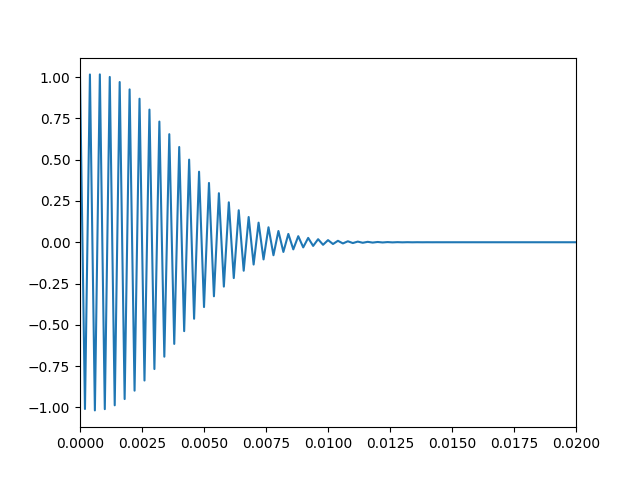
\includegraphics[width = 12cm]{eu_osc.png}
\end{center}
La dérivée est très grande et engendre des oscillations dues au dépassement des $y_i$ de chaque coté de 0.
\end{Answer}
%--------------------------------------------------------------------------
%--------------------------------------------------------------------------
%--------------------------------------------------------------------------
\section{Modifications de la méthode d'Euler}
%--------------------------------------------------------------------------
%--------------------------------------------------------------------------
%--------------------------------------------------------------------------
\subsection{Schéma de Heun}
%--------------------------------------------------------------------------
%--------------------------------------------------------------------------
Le schéma de Heun améliore le schéma d'Euler en s'inspirant du calcul d'une intégrale par la méthode des trapèzes : $\displaystyle \int_{a}^b g(u) \d u\simeq (b-a)\frac{g(a)+g(b)}2$. On obtient

\[ y(t_{k+1})-y(t_k)\simeq  (t_{k+1}-t_k) \frac {\varphi\bigl(y(t_k),t_k\bigr)+\varphi\bigl(y(t_{k+1}),t_{k+1}\bigr)}2 \]

Cependant cela devient une équation implicite en $y(t_{k+1})$ qu'on ne souhaite pas résoudre.

On va donc procéder en approchant la valeur de $y(t_{k+1})$ dans le second membre par celle que calcule la méthode d'Euler.
\begin{itemize}
\item On calcule $z_k=y_k+\varphi(y_k,t_k)(t_{k+1}-t_k)$ comme valeur approchée de $y(t_{k+1})$
\item On calcule la valeur approchée $\displaystyle y_{k+1} = y_k +
\frac{\varphi(y_k,t_k)+\varphi(z_k,t_{k+1})} 2 (t_{k+1}-t_k)$.
\end{itemize}
%--------------------------------------------------------------------------
%--------------------------------------------------------------------------
\begin{Exercise}\it
Écrire une fonction \type{heun(phi, y0, T)} qui implémente le schéma de Heun.
\end{Exercise}
%--------------------------------------------------------------------------
\begin{Answer}
\begin{lstlisting}
def heun(phi, y0, T):
    n = len(T)
    Y = [0]*n
    Y[0] = y0 
    for i in range(n-1):
        y = Y[i]
        pas = T[i+1] - T[i]
        pente_g = phi(y, T[i])
        z = y + pas*pente_g
        pente_d = phi(z, T[i+1])
        pente = (pente_g  + pente_d)/2
        Y[i+1] = y + pas*pente
    return Y
\end{lstlisting}
\newpage
\end{Answer}
%--------------------------------------------------------------------------
%--------------------------------------------------------------------------
\begin{Exercise}\it
Utiliser le schéma de de Heun pour résoudre $(t+1)y'(t)+y(t)=e^t$, $y(0)=1$ sur $[0;2]$ avec 5, 10 et 20 points.
La solution exacte est $t\mapsto \frac{e^t}{t+1}$.
\end{Exercise}
%--------------------------------------------------------------------------
\begin{Answer}
\begin{lstlisting}
def phi4(y, t) :
    return (m.exp(t) - y )/(t+1)

def f4(t) :
    return m.exp(t)/(t+1)

y0 = 1
t_max = 5

for n in [10, 100]:
    T = listeT(0, t_max, n)
    Y = heun(phi4, 1, T)
    plt.plot(T, Y, label='avec {} points'.format(n))
T = listeT(0, t_max, 1000)
Y = appliquer(f4, T)
plt.plot(T, Y, label = 'Solution exacte')
plt.legend()
plt.show()
\end{lstlisting}
\end{Answer}
%--------------------------------------------------------------------------
%--------------------------------------------------------------------------

\medskip

On revient à l'équation $y'=y$ sur $[0;1]$ avec $y(0)=1$.
%--------------------------------------------------------------------------
%--------------------------------------------------------------------------
\begin{Exercise}[title = {Qualité de l'approximation}]\it
Écrire les instructions qui permettent d'afficher à l'écran la valeur absolue entre \type{m.exp(1)} et le dernier terme de la liste retournée par la fonction \type{heun} pour des listes de $10^p$ points avec $p\in \{1, 2, 3, 4, 5,6, 7\}$.
\end{Exercise}
%--------------------------------------------------------------------------
\begin{Answer}
\begin{lstlisting}
y0 = 1
t_max = 1
for k in range(1, 8):
    n = 10**k
    T = listeT(0, t_max, n)
    Y = heun(phi1, y0, T)
    err = abs(m.exp(t_max) - Y[-1])
    print("Erreur : {} pour {} points".format(err, n))
\end{lstlisting}
L'erreur diminue d'un facteur 100 chaque fois qu'on multiplie par 10, sauf à la fin où les erreur d'arrondis ne permettent plus d'augmenter la précision des calculs. 
\end{Answer}
%--------------------------------------------------------------------------
%--------------------------------------------------------------------------
\subsection{Équations d'ordre 2}
%--------------------------------------------------------------------------
%--------------------------------------------------------------------------
On peut utiliser le principe du schéma d'Euler pour résoudre des équations d'ordre 2 (ou plus).

Ce sont des équations de la forme $y'' = \psi(y, y', t)$.

Par exemple l'équation $y'' + y' + ty = \sin(t)$ sera définie par

\begin{lstlisting}
def psi0(y, v, t):
    return m.sin(t) - v - t*y
\end{lstlisting}



Les conditions initiales seront données sous la forme $y(t_0) = y_0$, $y'(t_0) = v_0$.

Le cas des conditions aux limites, $y(t_0) = y_0$ et $y(t_{final}) = y_{final}$, plus difficile, ne sera pas traité ici.

On peut résoudre ces équations en suivant le même principe que dans le cas des équations d'ordre 1 en incluant le calcul des dérivées aux temps $t_i$. On cherchera donc à définir deux listes \type{Y}, pour les valeurs de la fonctions, et \type{V}, pour les valeurs de sa dérivée. La valeur de \type{Y[i]}, $y_i$, et celle de $V[i]$, $v_i$ seront des valeurs approchées de $f(t_i)$ et $f'(t_i)$ respectivement où $f$ est la solution telle que $f(t_0) = y_0$ et $f'(t_0)= v_0$.

Le schéma d'Euler se décompose alors en deux calculs. On note $\delta_i = t_{i+1} - t_i$ :
  \[y_{i+1}\simeq f(t_{i+1}) \simeq f(t_i) + \delta_i f'(t_i)  \simeq y_i + \delta_i v_i\hbox{ et }\]
  \[v_{i+1}\simeq f'(t_{i+1}) \simeq f'(t_i) + \delta_if''(t_i) = f'(t_i) + \delta_i\psi\bigl(f(t_i), f'(t_i),  t_i\bigr)\simeq v_i + \delta_i\psi(y_i, v_i, t_i)\]
%-------------------------------------------------------------------------------
%-------------------------------------------------------------------------------
\begin{Exercise}\it
Écrire une fonction \type{Euler2(phi, y0, v0, T)} qui résout une équation différentielle d'ordre 2 définie par $\psi$ avec les conditions initiales $y_0$ et $v_0$ en $t_0$ aux points définis par la liste des temps \type{T}. La fonction renverra deux listes de même taille que \type{T}, la première contiendra les valeurs approchées de la solution, l'autre les valeurs approchées de sa dérivée.
\end{Exercise}
%-------------------------------------------------------------------------------
\begin{Answer}
\begin{lstlisting}
def Euler2(psi, y0, v0, T):
    n = len(T)           
    Y = [0]*n 
    Y[0] = y0 
    V = [0]*n 
    V[0] = v0 
    for i in range(n-1): 
        pas = T[i+1] - T[i]
        Y[i+1] = Y[i] + pas*V[i]
        V[i+1] = V[i] + pas*psi(Y[i], V[i], T[i])
    return Y, V 
\end{lstlisting}
\newpage
\end{Answer}
%--------------------------------------------------------------------------
%--------------------------------------------------------------------------
\subsection{Schéma de Runge-Kutta}
%--------------------------------------------------------------------------
%--------------------------------------------------------------------------
La méthode de Runge-Kutta s'inspire de la méthode de Simpson : 

\[ \int_{a}^b g(u) \d u\simeq (b-a)\frac{g(a)+4g\bigl(\frac{a+b}2\bigr)+g(b)}6\]

On obtient, pour $m_k = \frac{t_k+t_{k+1}}2$ et $h=t_{k+1}-t_k$,

\[ y(t_{k+1})\simeq y(t_k) + h \frac {\varphi\bigl(y(t_k),t_k\bigr)+4\varphi\bigl(y(m_k),m_k\bigr) + \varphi\bigl(y(t_{k+1}),t_{k+1}\bigr)}6 \]


Comme dans la méthode de Heun, on calcule des valeurs de de $y(m_k)$ et $y(t_{k+1})$ par des approximations simples ; en fait on calcule deux approximations de $y(m_k)$.


\begin{itemize}
\item $a = y_k+\frac{h}2 \varphi\bigl(y_k,t_k\bigr)$ est une première valeur approchée de $y(m_k)$,

\item $ b = y_k + \frac{h}2 \varphi\bigl(a, t_k+\frac h2\bigr)$ est aussi une valeur approchée de $y(m_k)$,

\item $c = y_k + h \varphi\bigl(b, t_k+\frac h2\bigr)$ est une valeur approchée de $y(t_{k+1})$.
\item 
\item On pose alors 

$\displaystyle  y_{k+1} = y_k+ h \frac{\varphi\bigl(y_k,t_k\bigr) + 2\varphi\bigl(a, t_k+\frac h2\bigr) + 2\varphi\bigl(b, t_k+\frac h2\bigr)  + \varphi\bigl(c, t_k+h\bigr)}6$
\end{itemize}
%--------------------------------------------------------------------------
%--------------------------------------------------------------------------
\begin{Exercise}[label={exo:RK}]\it
Écrire une fonction \type{RK(phi, y0, T)} qui donne une approximation de la solution de $y' = \varphi(y, t)$ avec la condition initiale $y(t_0)=y_0$ aux points de la liste $T$ par la méthode de Runge-Kutta.
\end{Exercise}
%--------------------------------------------------------------------------
\begin{Answer}
\begin{lstlisting}
def RK(f, y0, T):
    n = len(T)
    Y = [0]*n
    Y[0] = y0 
    for i in range(n-1): 
        y = Y[i]
        t = T[i]
        t1 = T[i+1]
        pas = t1 - t
        pente1 = f(y,t)
        a = y + pente1*pas/2   # 1ère valeur au milieu
        pente2 = f(a, t+pas/2) # 1ère pente au milieu
        b = y + pente2*pas/2   # 2ème valeur au milieu
        pente3 = f(b, t+pas/2) # 2ème pente au milieu
        c = y + pente3*pas     # valeur à droite
        pente4 = f(c,t1)       # pente à droite
        pente = (pente1 + 2*pente2 + 2*pente3 + pente4)/6
        Y[i+1] = y + pas*pente
    return Y
\end{lstlisting}
\end{Answer}
%--------------------------------------------------------------------------
%--------------------------------------------------------------------------
\subsection{Schéma d'Euler implicite}
%--------------------------------------------------------------------------
%--------------------------------------------------------------------------
La formule d'approximation utilisée : $f(x_{i+1}) \simeq f(x_i) + (x_{i+1} - x_i) f'(x_i)$ peut être lue dans le sens inverse : 
$f(x_i) \simeq f(x_{i+1}) + (x_i - x_{i+1}) f'(x_{i+1}) = f(x_{i+1}) + (x_i - x_{i+1})\varphi\bigl(f(x_{i+1}, x_{i+1}\bigr)$. En remplaçant les valeurs par leurs valeurs approchées on aboutit au schéma d'Euler implicite
\[y_{i} =  = y_{i+1}+ (t_i -t_{i+1}) \varphi(y_{i+1},t_{i+1})\]

On voit qu'on ne peut pas directement exprimer $y_{i+1}$ en fonction de $y_i$ ;  il faut résoudre, à chaque étape, l'équation $g_i(y)=0$ avec $g_i(y)= y + (t_i -t_{i+1}) \varphi(y_{i+1},t_{i+1}) - y_i$.

\medskip

Dans certains cas, rares, cela est possible simplement.

Par exemple si on veut résoudre l'équation différentielle $y'=y^2+t^2$ pour $y(t_0)=y_0$ sur $[t_0;t_1]$ par la méthode d'Euler implicite, on doit doit calculer les $y_i$ à partir de $y_0$ et $y_i = y_{i+1}  + (t_i - t_{i+1}) \bigl(y_{i+1}^2+t-{i+1}^2\bigr)$.

Ainsi $y_{i+1}$ est racine d'un polynôme de degré 2 : on choisira la racine proche de $y_i$.
%--------------------------------------------------------------------------
\begin{Exercise}[label={exo:RK}]\it
Écrire une fonction \type{implicite(y0, T)} qui donne une approximation de la solution de $y' = y^2 + t^2$ avec la condition initiale $y(t_0)=y_0$ aux points de la liste $T$ à l'aide du schéma d'Euler implicite.

On notera que cette fonction ne sait résoudre qu'une seule équation.
\end{Exercise}
%--------------------------------------------------------------------------
\begin{Answer}
Les racines sont $\displaystyle \frac{1\pm\sqrt{1-4hy_i-4h^2t_{i+1}^2}}{2h}$ avec $ h = t_{i+1} - t_i$ ;

celle qui est proche de $y_i$  est
$\displaystyle \frac{1-\sqrt{1-4hy_i-4h^2t_{i+1}^2}}{2h}$.

\smallskip


%--------------------------------------------------------------------------
\begin{lstlisting}
def implicite(y0, T):
    n = len(T)
    Y = [0]*n 
    Y[0] = y0
    for i in range(n-1): 
        pas = T[i+1] - T[i]
        delta = 1 - 4*pas*(Y[i]+pas*T[i+1]**2)
        Y[i+1] = (1-delta**(1/2))/(2*h)
    return Y
\end{lstlisting}
\end{Answer}
%--------------------------------------------------------------------------
%--------------------------------------------------------------------------

\medskip

Dans le cas général on peut utiliser la fonction \type{fsolve} du module \type{scipy.optimize} pour résoudre l'équation en $y_{i+1}$. On devra, à chaque étape, définir une nouvelle fonction qu'il faudra envoyer comme paramètre à \type{fsolve}. On prendra $y_i$ comme valeur initiale.
%--------------------------------------------------------------------------
%--------------------------------------------------------------------------
\begin{Exercise}[label={exo:impl}]\it 
Écrire une fonction \type{eulerImplicite(phi, y0, T)} qui donne une approximation de la solution de $y' = \varphi(y, t)$ avec la condition initiale $y(t_0)=y_0$ aux points de la liste $T$ par la méthode d'Euler implicite.
\end{Exercise}
%--------------------------------------------------------------------------
\begin{Answer}

\begin{lstlisting}
from scipy.optimize import fsolve 

def eulerImplicite(phi, y0, T) :
    n = len(T)
    Y = [0]*n
    Y[0] = y0 
    for i in range(n-1): 
        # On féfinit une fonction dans la fonction
        def g(x): 
            return x - Y[i] - (T[i+1]-T[i])*phi(x, T[i+1])
        Y[i+1] = fsolve(g,Y[i])  
    return Y
\end{lstlisting}
\end{Answer}
%--------------------------------------------------------------------------
%--------------------------------------------------------------------------

